\section{Spring}
\label{subsec:spring}

\begin{figure}[H]
    \centering
    
\includegraphics[scale=0.11]{images/spring.png}
    \caption{Logotipo da framework Spring.}
    \label{fig:spring}
\end{figure}

\hspace{5mm} A \href{https://spring.io/}{Spring} é uma framework desenvolvida pela equipa \href{https://pivotal.io/}{pivotal} usando Java dedicada principalmente à implementação de lógica aplicacional back-end.

\subsection{Vanatagens}

\hspace{5mm} Existem enúmeras vantagens ao utilizar esta framework tais como:

\begin{itemize}
    
    \item é \textbf{escrita em Java}, beneficiando do facto de ser uma linguaguem muito usada e preparada para projetos de elevada complexidade (usando conceitos de POO). Outra vantagem da utilização de Java é a comunidade (tanto documentação oficial como tutoriais e explicações de terceiros) ser grande e consistente, tornando o suporte a dúvidas e obstáculos do desenvolvimento mais facilitados de se superar.
    
    \item diversos desenvolvedores fidedignos, tais como: Alibaba, Amazon, Google, Microsoft, entre outros; \textbf{confiam na framework}, sendo um indicador positivo a favor da utilização da mesma. 
    
    \item é uma framework \textbf{flexivel} uma vez que a sua arquitetura base utiliza os padrões \href{https://en.wikipedia.org/wiki/Inversion_of_control}{Inversion of Control (IoC)} e \href{https://en.wikipedia.org/wiki/Dependency_injection}{Dependency Injection (DI)} tornando a implementação do código facilitada uma vez que parte considerável da lógica é automaticamente introduzida.
    
    \item contém inúmeras \textbf{bibliotecas de terceiros} integradas na arquitetura base constituindo um conjunto de ferramentas disponível para qualquer tipo de aplicação tanto server-side como client-side. Por exemplo a framework \href{https://hibernate.org/}{hibernate} é facilmente integrada no modelo de dados de uma API RESTful já escrita em Spring, tornando o processo de presistência de dados intuitivo e praticamente automático.  
    
    \item contém o \textbf{plugin} \href{https://spring.io/projects/spring-boot}{Spring boot} que automatiza a criação da infaestrutura inicial do projeto: inicializando e configurando o servidor aplicacional \href{http://tomcat.apache.org/Tomcat}{Tomcat}, verifica e descarrega bibliotecas necessárias para o contexto da aplicação e disponibiliza métricas para avaliar o desempenho e estado do sistema, podendo ser remotamente avaliado.
    
    \item é uma framework \textbf{segura}. Utilizar bibliotecas de terceiros é sempre um risco uma vez que os seus desenvolvedores podem simplesmente desistir e descontinuar atualizações das bibliotecas ficando as mesmas sem suporte e sujeitas a vulnerabilidades ou erros. Desta forma a equipa da Spring monotoriza e verifica o estado das bibliotecas terceiras integradas na sua arquitetura certificando que o seu uso é seguro.
    
    \item por último mas não menos importante a Spring, tal como Java, tem uma \textbf{comunidade grande e prestável} com ínumeros tutoriais e artigos na própria documentação oficial.
\end{itemize}


\subsection{Arquitetura}

\begin{figure}[H]
    \centering
    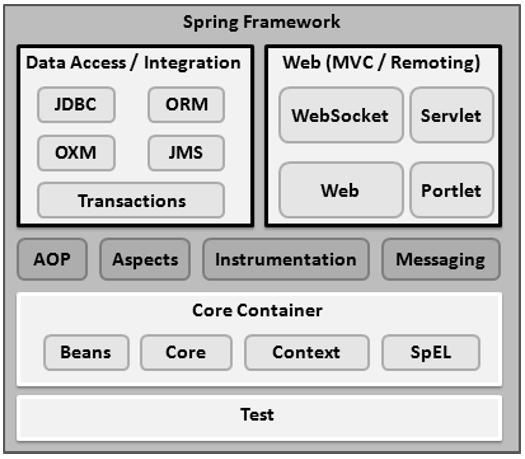
\includegraphics[scale=0.8]{images/spring_architecture.png}
    \caption{Arquitetura da framework Spring.}
    \label{fig:grails}
\end{figure}

\subsubsection{Core Container}

\hspace{5mm} O Core Container contém as principais classes que formam a arquitetura base da framework.

\begin{itemize}
    
    \item O módulo Core contém a implementação dos padrões arquiteturais: IoC e DI; referidos anteriormente.
    
    \item O módulo Bean implementa o padrão Factory (usado para criação genérica de obejtos), neste caso é uma fábrica de Beans.
    
    \item O módulo Context utiliza os módulos Core e Bean para gerar automaticamente os objetos configurados pela implementação específica do programador. 
    
    \item O módulo SpEL é utilizado pela Spring para gerar gráficos e monotorizar os objetos gerados e configurados pela própria framework.
    
\end{itemize}

\subsubsection{Outros Containers}

\hspace{5mm} O container Data Access implementa as classes necessárias ao acesso e manipulação de dados nas diferentes base de dados existentes.

\hspace{5mm} O container Web implementa o padrão MVC utilizado para responder a pedidos HTTP ou outros protocolos.


\subsection{Exemplo prático}

\hspace{5mm} Nesta secção segue-se um exemplo prático no qual foi criada uma API RESTful expondo a lógica back end através de métodos HTTP.

\subsubsection{Model - classe Person}

\hspace{5mm} Incialmente definiu-se uma classe Person que representa a informação de uma Pessoa, contendo o seu id, nome, idade e email. A vermelho em cima da declaração de cada variével de instância é possível observar \textbf{anotações}. 

\begin{figure}[H]
    \centering
    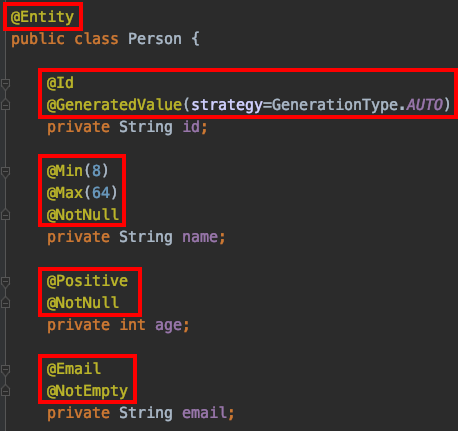
\includegraphics[scale=0.6]{images/Person_variables.png}
    \caption{Model Person.}
    \label{fig:grails}
\end{figure}

\begin{itemize}
    
    \item @GeneratedValue(...) - indica que a variável id é gerada automaticamente pela framework, neste caso é uma sequência de inteiros começado em 1 em formato String.
    
    \item @Min(8) - indica que a string (nome) tem de ter no mínimo 8 caracteres.
    
    \item @Max(64) - indica que a string (nome) tem de ter no máximo 64 caracteres.
    
    \item @NotNull - indica que a variável tem de ter necessáriamente um valor.
    
    \item @NotEmpty - indica que a variável tem de ter necessáriamente um valor não vazio.
    
    \item @Positive - indica que o inteiro (idade) tem de ser positivo.
    
    \item @Email - indica que a string tem de ter um formato válido de email.
    
\end{itemize}

\hspace{5mm} Existem outras anotações o importante é que a Spring juntamente com a framework hibernate integrada, valida automaticamente os valores atribuídos no momento de criação do objeto Person, lançando uma excepção quando os mesmos são inválidos.

\hspace{5mm} A anotação \textbf{@Entity} indica á hibernate que a classe refere-se a uma tablela na base de dados. A anotação \textbf{@Id} indica que a variável id é chave primária nessa mesma tabela.

\subsubsection{Controller - classe PersonController}

\hspace{5mm} Tendo definido o modelo de dados (classe Person) é necessário definir a classe que implementa os métodos que processam, neste caso, os pedidos HTTP associados a este objeto, a classe PersonController.


\begin{figure}[H]
    \centering
    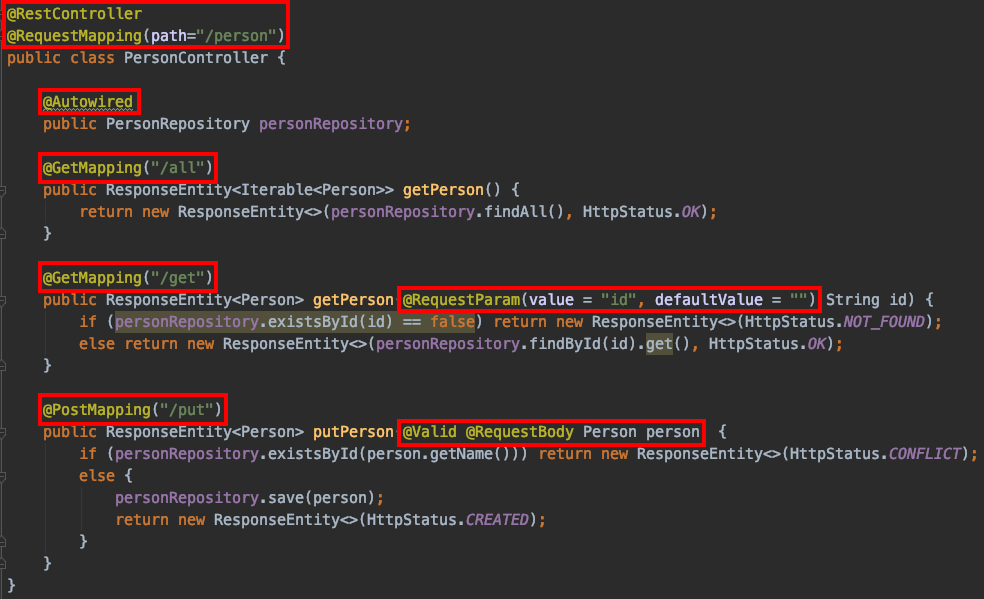
\includegraphics[scale=0.5]{images/PersonController.png}
    \caption{Controller PersonController.}
    \label{fig:grails}
\end{figure}

\begin{itemize}
    
    \item @RestController indica à Spring que esta classe é um Controller e por isso de acordo com o mapeamento das rotas pode processar HTTP Requests.
    
    \item RequestMapping(...) indica o nome da rota (no url) para evocar este controlador.
    
    \item @GetMapping(...) indica que este método processa HTTP GETs evocados pela rota definida no url.
    
    \item @PostMapping(...) indica que este método processa HTTP POSTs evocados pela rota definida no url.
    
    \item @Valid tal como referido anteriomente é utilizado para validar os dados introduzidos na classe model (neste caso Person). 
    
    \item @RequestBody indica que o objeto em causa foi exportado do payload (body) do pedido HTTP.
    
    \item @RequestParam indica que a variável em causa corresponde a um parâmetro específico do pedido HTTP.
    
    \item @Autowired é uma das anotações mais importante e eficaz, indica à framework hibernate que o objeto (neste caso PersonRepository) que é responsável pela persisntência dos dados (DAO) é automaticamente gerado e criado (criação dinâmica do objeto), sem qualquer intervenção do programador.
    
\end{itemize}

\subsubsection{DAO - interface PersonRepository}

\hspace{5mm} Esta interface provavelmente é a que demonstra de forma mais óbvia o poder de utilizar uma framework no sentido da \textbf{simplicidade e automação} de desenvolvimento de código.

\begin{figure}[H]
    \centering
    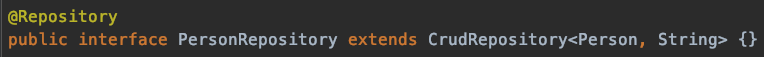
\includegraphics[scale=0.5]{images/PersonRepository.png}
    \caption{DAO PersonRepository.}
    \label{fig:grails}
\end{figure}

\hspace{5mm} Tal como se observa na figura, apenas indicando que a interface é do tipo CrudRepository e refere-se ao modelo de dados Person, a Spring juntamente com o Hibernate gera e cria dinâmicamente uma classe que implementa esta interface fazendo a ligação entre os modelos e a sua preseistência na base de dados.

\subsection{Análise final}

\hspace{5mm} Em suma, a criação das respetivas classes: Model, Controller e DAO; tornam-se simples e intuitiva uma vez que a Spring juntamente com as bibliotecas de terceiros integradas automatizam e gerem dinamicamente classes e dependências necessárias. 